\subsection{Etapa de Aislación de Señal}

Ahora se debe implementar un circuito auxiliar que provea una aislación galvánica entre los componentes que se sitúan del lado de potencia de la plataforma (como los transistores, diodos, circuito driver, etc.), y los componentes de la parte digital del sistema (como el controlador digital de señales, el circuito de acondicionamiento, etc.).\\

Existen tres partes principales de la plataforma, donde se pasa de la parte digital a la de potencia, donde se requiere algún tipo de aislación:\\

\begin{enumerate}
    \item Entre las salidas PWM del controlador y las entradas de comando de los drivers 2ED21834-S06J de la figura \ref{circuito_driver}.
    \item Para las líneas del bus I\textsuperscript{2}C que comunican al sensor LM5056A de la figura \ref{conexion_LM5056A} (lado de potencia) con el módulo I\textsuperscript{2}C del controlador.
    \item Para la medición de corriente de salida mediante el sensor de efecto Hall TMCS1100A4 de la figura \ref{conexion_TMCS1100}.
    \item Para generar fuentes de alimentación aisladas para los circuitos del lado digital.\\
\end{enumerate}

En este capítulo vamos a tratar las soluciones de aislación para los primeros dos casos. En el tercer caso, el TMCS1100A4, al ser un dispositivo que funciona por medio del efecto Hall, ya tiene aislación incluida en su diseño, por lo que la salida del mismo ya se encuentra aislada del convertidor. Para el cuarto ítem, esto se va a tratar propiamente y en profundidad en la sección de este capítulo dedicada a los circuitos de alimentación de la plataforma.\\

\subsubsection{Tecnologías de Aislación de Señal}

{\Bold\scshape Falta completar esta sección.}\\

\lipsum[1]\\

\subsubsection{Aislación de los Drivers}

Cómo los drivers están conectados directamente a terminales de los transistores de potencia del convertidor, estos se encuentran dentro de la etapa de potencia de la plataforma. Sin embargo, las señales PWM que definen el tiempo y secuencia de conmutación de los transistores provienen del módulo PWM del controlador digital, todo dentro del área digital de la plataforma. Entonces, previo a las entradas de señal de los 2ED21834-S06J se debe interponer algun circuito de aislación de señal, para mantener la separación entre las partes de potencia y digitales.\\

Los requerimientos que la aplicación exige del circuito aislador se presentan en la siguiente lista.\\

\begin{itemize}
    \item Retardo de propagación mucho menor al período $T_s$ de \SI[]{50}[]{\micro\second} de las ondas PWM de excitación.
    \item Tensión pico máxima de aislación superior a los \SI[]{100}[]{\volt}.
    \item Niveles lógicos de salida compatibles con las entradas de los drivers.
    \item Es deseable la utilización de encapsulados pequeños de montaje superficial.\\
\end{itemize}

Para este propósito se eligió utilizar el modelo {\Medium ACPL-P480} de Broadcom, un optoacoplador de un solo canal de alta velocidad, con un \textit{Schmitt trigger} que elimina la necesidad de circuitos externos para acondicionamiento de formas de onda. Algunos de sus parámetros más importantes se muestran en la tabla \ref{tabla:ACPL-P480}.\\

\setlength{\tabcolsep}{7pt}
\renewcommand{\arraystretch}{1.5}
\begin{table}[H]
\begin{center}
    \begin{tabular}{llrrrr}
    {\SemiBold Fabricante} & {\SemiBold Modelo} & $\mathbf{V_{ISO}}$ [\unit{\volt}] & $\mathbf{t_{PHL}}$ [\unit{\nano\second}] & $\mathbf{t_{PLH}}$ [\unit{\nano\second}] & $\mathbf{PWD}$ [\unit{\nano\second}]\\
    \hline
    Broadcom & ACPL-P480 & \num{3750} & \num{150} &  \num{110} & \num{250}
    \end{tabular}
    \caption{Especificaciones del optoacoplador modelo ACPL-P480 de Broadcom.\textsuperscript{\cite{ACPL-P480}}}
    \label{tabla:ACPL-P480}
\end{center}
\end{table}

Dónde $V_{ISO}$ es la máxima tensión momentánea soportada entre entrada y salida, $t_{PHL}$ es el retardo de propagación para una transición a nivel lógico bajo, $t_{PLH}$ es el retardo de propagación para una transición a nivel lógico alto, y $PWD$ es la distorsión de ancho de pulso, definida como $|t_{PHL} - t_{PLH}|$.\\

Este dispositivo viene en un empaquetado SMD de seis pines tipo \textit{stretched SO-6} o SO-6 estirado, como el de la figura \ref{encapsulado_opto}...\\

\begin{figure}[h]
    \centering
    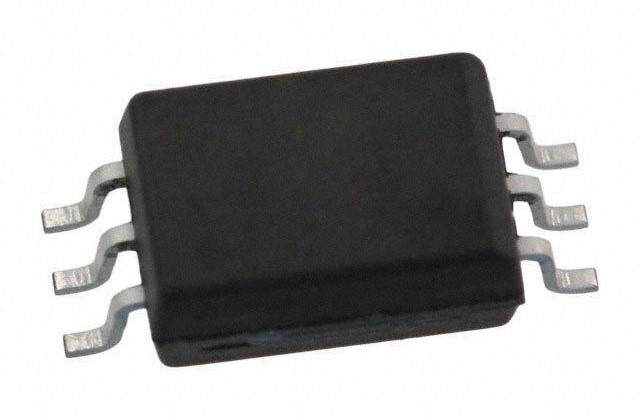
\includegraphics[scale=0.2]{Imagenes/SO6 Stretched.jpeg}
    \caption{Optoacoplador modelo ACPL-P480 de Broadcom, en su encapsulado SMD tipo SO-6 stretched.}
    \label{encapsulado_opto}
\end{figure}

\subsubsection{Aislación I\textsuperscript{2}C}

\lipsum[2]\\

